
%This thesis uses sequential composition of memoryless, continuous state feedback
%control policies to enable global navigation while respecting local constraints.  The
%thesis also enables more flexible planning on constrained systems.  

This chapter presents extensions to the basic sequential composition technique
described in~\cite{bur_riz_kod_99}.  These extensions allow for more general policy
types and prepares relationships, thereby increasing the flexibility of the approach.
General definitions that help formalize the discussion are given; model specific
details are withheld until Chapters~\ref{chap:fully} and~\ref{chap:nonholo}.  This
chapter defines the requirements for ``composable'' policies that later guide the
development of the feedback policies.

The chapter's first section gives general definitions and notation used throughout
the thesis.  The second section briefly describes the use of \emph{flow-through}
policies.  The chapter's third section describes four policy requirements that are
necessary for composable policies.  The focus is on the high-level requirements;
later chapters deal with the specific requirements of various robot models and
specific policy designs.  The fourth section discusses the basic approaches to
planning in the space of control policies.  This section serves to highlight the
issues and trade-offs involved in several approaches by focusing on a simple example.


\subsection{Extended Prepares Definition}
\label{sec:extended_prepares}

Sequential composition, as defined by~\cite{bur_riz_kod_99}, specifies a relationship
among the policies.  Finite time convergence coupled with conditional positive
invariance induces a transition relation between a given policy domain and the domain
of another policy which contains the goal set of the first policy.  Recall from
\resec{related_basicseqcomp}, that this pairwise relation between policies is called
a \emph{prepares} relationship, denoted $\CP_j \succeq \CP_i$~\cite{bur_riz_kod_99}.
In order to induce a prepares relationship with $\CP_i$, the size of the goal set of
$\CP_j$ is necessarily limited because the goal set must be contained in the domain
of $\CP_i$, which is a bounded region.

  
%Often the size of a policy domain that satisfies the policy
%requirements is tied to the size of its specified goal set; that is,
%larger goal sets tend to allow larger domains since the size of the
%domain for a given policy is limited by the system constraints.  To
%enable larger domains
To provide more flexibility in planning, it is useful to consider larger goal sets
not covered by a single policy domain.  Therefore, we extend the conventional
definition of \emph{prepares} from a relation between two policies, to a relation
between a policy and a set of policies.  
\begin{definition}{\bf Prepares:}
 A selected policy, $\CP_i$, \emph{prepares} a set of policies if
the goal set of the selected policy, $\Go{\CP_i}$, is contained in the
union of the domains of the policies in the set.  That is, $\CP_i
\succeq \crl{\CP_j}$ if $\Go{\CP_i} \subset \union_j \Do{\CP_j}$. 
\label{def:prepares}
\end{definition}
An example is shown in \refig{approach_nondeter}-a.

%% \addtolength{\floatsep}{-2ex}
%% \addtolength{\textfloatsep}{-2ex}
%% \addtolength{\dblfloatsep}{-2ex}
%% \addtolength{\dbltextfloatsep}{-2ex}
\begin{figure}[bt]
  \centering 
\begin{minipage}{0.45\linewidth}
  \centering 
\psfrag{P1}[]{\textcolor{red}{$\CP_A$}}
\psfrag{P2}[]{\textcolor{blue}{$\CP_B$}}
\psfrag{P3}[]{\textcolor{DarkGreen}{$\CP_C$}}
\psfrag{P4}[]{$\CP_D$}

  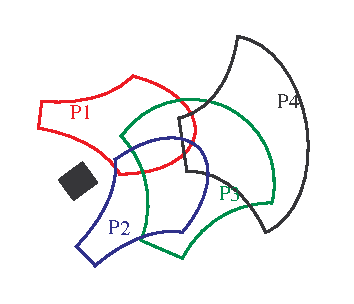
\includegraphics[width=\linewidth]{graphics/nondeter2D.eps} 

{\footnotesize (a)}
\end{minipage}
\hspace{0.05\linewidth}
\begin{minipage}{0.45\linewidth}
  \centering 
\psfrag{P1}[]{\textcolor{red}{$\CP_A$}}
\psfrag{P2}[]{\textcolor{blue}{$\CP_B$}}
\psfrag{P3}[]{\textcolor{DarkGreen}{$\CP_C$}}
\psfrag{P4}[]{$\CP_D$}
  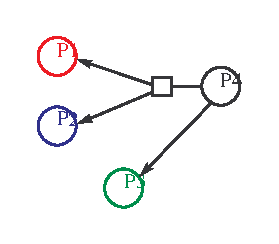
\includegraphics[width=\linewidth]{graphics/nondeterGraph.eps} 

{\footnotesize (b)}
\end{minipage}
 
\caption[Extended prepares definition]{Example of the extended
  prepares definition using iconic funnels.  a) Policy $\CP_D$
  prepares neither $\CP_A$ nor $\CP_B$, but does prepare $\CP_A \union
  \CP_B$ and $\CP_C$. b) Transition relation.  From the discrete
  planning perspective, the choice of transition from $\CP_D$ to
  $\CP_A$ or $\CP_B$ is non-deterministic; that is, it is imposed
  \emph{externally} by the closed-loop system dynamics.  The discrete
  planning method must account for either possibility.}

  \label{fig:approach_nondeter} 

\end{figure}
%% \addtolength{\floatsep}{2ex}
%% \addtolength{\textfloatsep}{2ex}
%% \addtolength{\dblfloatsep}{2ex}
%% \addtolength{\dbltextfloatsep}{2ex}

This added flexibility in the definition of prepares introduces added complexity to
the discrete transition relation encoded in the prepares graph.  Thus, the ability to
define larger goal sets via the extended prepares definition bears a cost that is
borne by the discrete planning.  The flow along a vector field is mathematically
determinate; therefore, from any initial condition within the single policy the flow
will result in a transition specific policies in the union. On the other hand, the
discrete transition relation encoded by the extended prepares relationship is an
approximation.  From the point of view of the discrete relationship, the transition
is non-deterministic, and cannot be represented by a simple graph.  The
nondeterminacy can be represented as an \emph{action} with multiple \emph{outcomes},
as shown in \refig{approach_nondeter}-b.  This representation is common with Markov
Decision Processes (MDP)~\cite{maxim_03,Wiki:MDP}.  From the perspective of the
discrete planning system, the choice of outcome is \emph{externally} imposed on the
discrete transition relation by the closed-loop system dynamics.
%once the hybrid control system choses an action based on its switching strategy.  
So long as the planning system takes each possible outcome into
account, the transition relation is valid for planning.  We will abuse
notation and continue to refer to the transition relation as a
``prepares graph'', even for the case of non-deterministic outcomes
induced by the extended prepares relationship.

%\FloatBarrier

\subsection{Policy Space Planning}
\label{sec:approach_planning}

This section highlights several issues involved in planning over a
collection of control policies that satisfy the above requirements.
Several approaches to defining switching strategies among the policies
are discussed; these approaches make use of existing discrete planning
techniques.  The discussion extends the basic partial order approach
presented in~\cite{bur_riz_kod_99}.  This thesis work enables advanced
planning techniques to be applied to systems with more complex
dynamics and constraints.

The planning takes place in the space of instantiated local feedback control
policies.  Recall from \resec{related_basicseqcomp}, that the \emph{palette} is a
collection of generic policies; that is policies with free parameters.  Policies are
\emph{instantiated} by assigning specific parameter values to a generic policy chosen
from the palette.  Given a collection of instantiated policies, which we call a
\emph{suite} of policies, planning involves defining a switching strategy among those
policies to address a given task.  The suite of policies and the switching strategy
is called a \emph{deployment}.


%% \addtolength{\floatsep}{-2ex}
%% \addtolength{\textfloatsep}{-2ex}
%% \addtolength{\dblfloatsep}{-2ex}
%% \addtolength{\dbltextfloatsep}{-2ex}
\begin{figure}[bt]
  \centering 
\begin{minipage}{0.85\linewidth}
  \centering 
\psfrag{P1}[]{\textcolor{red}{ $\CP_A$}}
\psfrag{P2}[]{\textcolor{blue}{ $\CP_B$}}
\psfrag{P3}[]{\textcolor{DarkGreen}{ $\CP_C$}}
\psfrag{P4}[]{\textcolor{black}{ $\CP_D$}}
\psfrag{P5}[]{\textcolor{blue}{ $\CP_E$}}
\psfrag{P6}[]{\textcolor{red}{ $\CP_F$}}
\psfrag{P7}[]{\textcolor{DarkGreen}{ $\CP_G$}}
\psfrag{P8}[]{\textcolor{blue}{ $\CP_H$}}
\psfrag{P9}[]{\textcolor{black}{ $\CP_I$}}
\psfrag{P10}[]{\textcolor{DarkGreen}{ $\CP_J$}}
\psfrag{P11}[]{\textcolor{blue}{ $\CP_K$}}
\psfrag{P12}[]{\textcolor{black}{ $\CP_L$}}
\psfrag{P13}[]{\textcolor{red}{ $\CP_M$}}
\psfrag{P14}[]{\textcolor{DarkGreen}{ $\CP_N$}}
\psfrag{P15}[]{\textcolor{blue}{ $\CP_O$}}
\psfrag{P16}[]{\textcolor{red}{ $\CP_P$}}
\psfrag{P17}[]{\textcolor{DarkGreen}{ $\CP_Q$}}
\psfrag{P18}[]{\textcolor{blue}{ $\CP_R$}}
\psfrag{P19}[]{\textcolor{black}{ $\CP_S$}}
\psfrag{P20}[]{\textcolor{red}{ $\CP_T$}}
\psfrag{P21}[]{\textcolor{black}{ $\CP_U$}}
\psfrag{P22}[]{\textcolor{DarkGreen}{ $\CP_V$}}
\psfrag{P23}[]{\textcolor{black}{ $\CP_W$}}
\psfrag{P24}[]{\textcolor{red}{ $\CP_X$}}
\psfrag{P25}[]{\textcolor{DarkGreen}{ $\CP_Y$}}
\psfrag{P26}[]{\textcolor{black}{ $\CP_Z$}}

  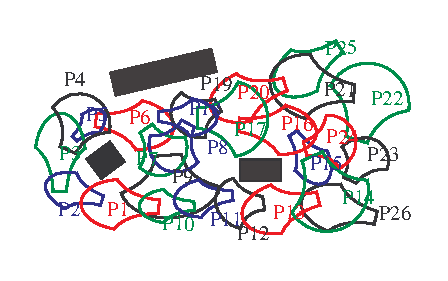
\includegraphics[width=\linewidth]{graphics/collection2D.eps} 

{\footnotesize (a)}
\end{minipage}

%\hspace{0.05\linewidth}

\begin{minipage}{0.85\linewidth}
  \centering 
\psfrag{P1}[]{\textcolor{red}{ $\CP_A$}}
\psfrag{P2}[]{\textcolor{blue}{ $\CP_B$}}
\psfrag{P3}[]{\textcolor{DarkGreen}{ $\CP_C$}}
\psfrag{P4}[]{\textcolor{black}{ $\CP_D$}}
\psfrag{P5}[]{\textcolor{blue}{ $\CP_E$}}
\psfrag{P6}[]{\textcolor{red}{ $\CP_F$}}
\psfrag{P7}[]{\textcolor{DarkGreen}{ $\CP_G$}}
\psfrag{P8}[]{\textcolor{blue}{ $\CP_H$}}
\psfrag{P9}[]{\textcolor{black}{ $\CP_I$}}
\psfrag{P10}[]{\textcolor{DarkGreen}{ $\CP_J$}}
\psfrag{P11}[]{\textcolor{blue}{ $\CP_K$}}
\psfrag{P12}[]{\textcolor{black}{ $\CP_L$}}
\psfrag{P13}[]{\textcolor{red}{ $\CP_M$}}
\psfrag{P14}[]{\textcolor{DarkGreen}{ $\CP_N$}}
\psfrag{P15}[]{\textcolor{blue}{ $\CP_O$}}
\psfrag{P16}[]{\textcolor{red}{ $\CP_P$}}
\psfrag{P17}[]{\textcolor{DarkGreen}{ $\CP_Q$}}
\psfrag{P18}[]{\textcolor{blue}{ $\CP_R$}}
\psfrag{P19}[]{\textcolor{black}{ $\CP_S$}}
\psfrag{P20}[]{\textcolor{red}{ $\CP_T$}}
\psfrag{P21}[]{\textcolor{black}{ $\CP_U$}}
\psfrag{P22}[]{\textcolor{DarkGreen}{ $\CP_V$}}
\psfrag{P23}[]{\textcolor{black}{ $\CP_W$}}
\psfrag{P24}[]{\textcolor{red}{ $\CP_X$}}
\psfrag{P25}[]{\textcolor{DarkGreen}{ $\CP_Y$}}
\psfrag{P26}[]{\textcolor{black}{ $\CP_Z$}}
\psfrag*{1}{{ $1$}}
\psfrag*{2}{{ $2$}}
\psfrag*{3}{{ $3$}}

  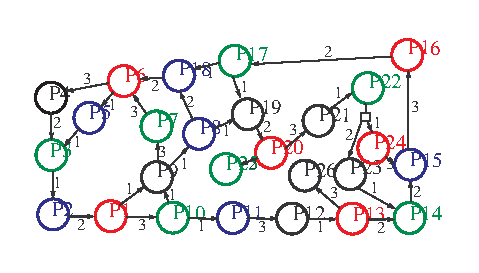
\includegraphics[width=\linewidth]{graphics/collectionGraph.eps} 

{\footnotesize (b)}
\end{minipage}

\caption[Example collection of policies and prepares graph]{Given the
  collection of iconic policies $\Lambda$ shown in (a), the discrete
  transition relation $\GL$ shown in (b) encodes the ``prepares''
  relationship between policies.  Thus the continuous behavior of the
  system is abstracted as a discrete set of transitions between policy
  domains.  Each transition shows an associated heuristic cost that
  may be used in planning.}

  \label{fig:approach_prepares} 

\end{figure}
%% \addtolength{\floatsep}{2ex}
%% \addtolength{\textfloatsep}{2ex}
%% \addtolength{\dblfloatsep}{2ex}
%% \addtolength{\dbltextfloatsep}{2ex}

To illustrate the types of planning that are possible on the discrete
prepares graph, consider the ``toy'' example shown in
\refig{approach_prepares}.  Here 26 policies are instantiated over the
workspace with three obstacles; these policies make up the suite
$\Lambda = \crl{\CP_A, \dots, \CP_Z}$.  The policy domains are shown
in \refig{approach_prepares}-a, and the associated prepares graph,
\GL, is shown in \refig{approach_prepares}-b.  The figure shows one
example of the extended prepares definition with $\CP_V \succeq
\crl{\CP_X, \CP_W}$.  Two policies, $\CP_Y$ and $\CP_Z$, do not
prepare any others.  As is generally the case, the prepares graph is
cyclic.

In the discussion that follows, some planning methods use a cost associated with each
transition to facilitate policy ordering.  In this example, a heuristic cost has been
assigned to each edge in the graph shown in \refig{approach_prepares}-b.  This
section does not address how the costs are assigned.
%, and instead assumes they are given.

In the subsequent discussion, the switching strategies are often
modeled as finite automata, with nodes and transitions between nodes.
For each node there is an associated policy that is executed upon
transition into the node.  Initially, there is a one-to-one
correspondence between nodes and policies; later, as temporal
dependencies are incorporated, the automata will have multiple nodes
that map to a single policy.  For this reason, this discussion will
enforce a distinction between a node in the automata representation
and its associated control policy.  Transitions represent switches
between policies governed by the continuous state evolution into the
domain of a policy associated with a child node; that is, the
transitions are enabled with the state enters the domain of a policy
associated with a child node.  

For transitions based on the extended prepares definition, the
transition will be associated with a non-deterministic outcome, and the
finite automata may more properly be modeled as a Markov Decision
process.  Here the transition is an action, with multiple outcomes.
The action represents a desired transition to a set of nodes
associated with the set of policies in the extended prepares.  The
transition is enables as soon as the system state enters the domain of
any policy associated with an outcome node.  This thesis will use the
term finite automata to encompass the non-deterministic outcomes.

For simple navigation to an overall goal, we assume the existence of a
single stabilizing policy, which will be referred to as the ``goal
policy.''  The node in the automaton that is associated with the goal
policy will be the termed the ``goal node.''  In some cases, where the
system has a known initial condition, references to the ``initial
policy'' and ``initial node'' are made as appropriate, where the
initial state is contained in the domain of the initial policy.

\subsection{Automata-based Planning}
\label{sec:automata}

In order to plan for higher-level task specification, including those
with the need to respond to events or respect temporal restrictions, a
more flexible planning approach is needed.  Sequence-based approaches
require replanning if the system needs to react to an event, and
order-based approaches by themselves are only suitable for single
tasks.  To address this issue, recent work has focused on
automatically synthesizing automata from a prepares
graph~\cite{belta_06,hadas_07}.

Combining policy composition with automata synthesis leverages the strengths of
control theoretic and computer science approaches.  Control theoretic approaches
offer provable guarantees over local domains; unfortunately, the control design
requires a low-level specification of the task.  In contrast, discrete planning
advances from computer science offer the ability to specify more general behaviors,
which may react to environmental changes, and generate verifiable solutions at the
discrete level; discrete planning lacks the continuous guarantees and robustness
offered by feedback.  Synthesizing an automaton that governs the execution of the
local feedback policies provides the benefits of both feedback and discrete planning,
while mitigating the drawbacks.  These automata synthesis tools specify behaviors in
terms of linear temporal logic (LTL) operations on the prepares graph nodes.  LTL
combines the standard Boolean logic operators, such as `AND',`OR', and `NOT', with
temporal operators such as 'ALWAYS' and 'NEXT'~\cite{Emerson}.

Kress-Gazit \ea~\cite{hadas_07} have developed an automaton synthesis tool that use
specifications encoded in a subset of the full LTL that describe behaviors on the
prepares graph generated by the work in this thesis.  The approach allows both
discrete inputs and discrete outputs to be specified.  The discrete inputs are sensed
by the robot, and the discrete outputs trigger actions, such as sound an alarm.  This
allows the system to change high-level behavior-based on discrete events, which
allows the system to react to environmental changes in a guaranteed manner.
Given a specification and prepares graph, the synthesis process either extracts an
automaton that satisfies the specification, or shows that the specification is not
realizable on the prepares graph.  Transitions in the automaton are governed by the
transitions between policy domains and the discrete events sensed by the
robot~\cite{dcchkg_07}.  Thus, the combination of automata and continuous feedback
control policies allows high-level specifications to be satisfied by executing the
continuous feedback control policies.  The work in this thesis has enabled these
approaches to be applied to more complex systems.


% Some LTL operators are
% shown in Table~\ref{table:LTL_ops}.
% \begin{table}
% \caption{Some standard LTL operators.}
% \centering
% \begin{tabular}{|c|c|}
% \hline
% `NOT' & $\NOT$\\
% `AND'&$\AND$\\
% `OR' &$\OR$\\
% `IMPLIES'& $\IMPLIES$\\
% `IF AND ONLY IF' & $\IFF$\\
% `NEXT' & $\NEXT$\\
% `ALWAYS' & $\ALWAYS$\\
% `EVENTUALLY' & $\EVENTUALLY$\\
% `UNTIL' &$\UNTIL$\\
% \hline
% \end{tabular}
% \label{table:LTL_ops}
% \end{table}


%% \addtolength{\floatsep}{-2ex}
%% \addtolength{\textfloatsep}{-2ex}
%% \addtolength{\dblfloatsep}{-2ex}
%% \addtolength{\dbltextfloatsep}{-2ex}
\begin{figure}[bt]%
  \centering 
\begin{minipage}{0.85\linewidth}
  \centering 
\psfrag{S}[]{$S$}
\psfrag{E}[]{Event `EV'}
\psfrag{G}[]{$G$}

  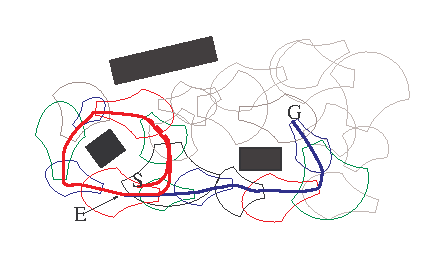
\includegraphics[width=\linewidth]{graphics/automaton2D.eps} 

{\footnotesize (a)}
\end{minipage}
%\hspace{0.05\linewidth}

\begin{minipage}{0.85\linewidth}
  \centering 
\psfrag{P1}[]{\textcolor{red}{ $\CP_A$}}
\psfrag{P2}[]{\textcolor{blue}{ $\CP_B$}}
\psfrag{P3}[]{\textcolor{DarkGreen}{ $\CP_C$}}
\psfrag{P4}[]{\textcolor{black}{ $\CP_D$}}
\psfrag{P5}[]{\textcolor{blue}{ $\CP_E$}}
\psfrag{P6}[]{\textcolor{red}{ $\CP_F$}}
\psfrag{P7}[]{\textcolor{DarkGreen}{ $\CP_G$}}
\psfrag{P8}[]{\textcolor{blue}{ $\CP_H$}}
\psfrag{P9}[]{\textcolor{black}{ $\CP_I$}}
\psfrag{P10}[]{\textcolor{DarkGreen}{ $\CP_J$}}
\psfrag{P11}[]{\textcolor{blue}{ $\CP_K$}}
\psfrag{P12}[]{\textcolor{black}{ $\CP_L$}}
\psfrag{P13}[]{\textcolor{red}{ $\CP_M$}}
\psfrag{P14}[]{\textcolor{DarkGreen}{ $\CP_N$}}
\psfrag{P15}[]{\textcolor{blue}{ $\CP_O$}}
\psfrag{IC}[]{IC}
\psfrag{NG}[cB]{$\neg\,\mrm{EV}$}
\psfrag{GD}[lt]{EV}

  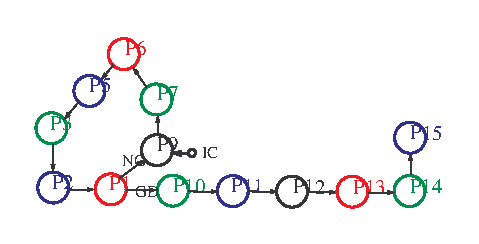
\includegraphics[width=\linewidth]{graphics/automatonGraph.eps} 

{\footnotesize (b)}
\end{minipage}

\caption[Automata-based planning]{ Automata-based planning allows for
  the system to react to local conditions while satisfying a given
  specification.   Figure (a) shows portions of the path taken while satisfying
  the automaton shown in (b).  }

  \label{fig:approach_automaton} 

\end{figure}
%% \addtolength{\floatsep}{2ex}
%% \addtolength{\textfloatsep}{2ex}
%% \addtolength{\dblfloatsep}{2ex}
%% \addtolength{\dbltextfloatsep}{2ex}

%\clearpage % just for this run

Returning to the example of \refig{approach_prepares}, we wish to specify that the
robot patrol the lower left obstacle until an event is seen, and then goes to a
particular station.  The first part, ``patrol
the lower left obstacle by visiting areas `F' and `A', until an event `EV' at `A' is
seen.''  
%, is given in LTL by $\prl{\prl{\ALWAYS\EVENTUALLY \CP_F \AND \ALWAYS\EVENTUALLY
%    \CP_A }\UNTIL \prl{\CP_A \AND \mrm{EV}}}$\footnote{There are two subtleties with this specification.  Due to
%  the formalism of the UNTIL operator, this particular formula is only
%  valid if ${\CP_A \AND \mrm{EV}}$ eventually becomes true; that is
%  the event eventually happens.  Also, we assume policy 'O' stops in
%  the goal set.}.  
After seeing the event, ``go to 'O', sound an  and stay put.''
% is given by
%$\ALWAYS\prl{\prl{\CP_A \AND \mrm{EV}} \Rightarrow \EVENTUALLY \CP_O}  \AND
%\ALWAYS\prl{\CP_O \Rightarrow \NEXT \CP_O}$.  At 'O', ``sound an alarm'' is encoded
%by $\ALWAYS\prl{\CP_O \Rightarrow `ALARM'}$.  All of these should be true for the
% complete system behavior, so they are combined to give the temporal logic formula 
% \begin{equation}
% \bba{c}
% \prl{\prl{\ALWAYS\EVENTUALLY \CP_F \AND \ALWAYS\EVENTUALLY
%     \CP_A }\UNTIL \prl{\CP_A \AND \mrm{EV}}}\\
% \AND\\
% \ALWAYS\prl{\prl{\CP_A \AND \mrm{EV}} \Rightarrow \EVENTUALLY \CP_O} \\
% \AND\\
% \ALWAYS\prl{\CP_O \Rightarrow \NEXT \CP_O} \\
% \AND\\
% \ALWAYS\prl{\CP_O \Rightarrow `ALARM'}
% \eba\,.
% \label{eqn:approach_LTL_spec}
% \end{equation}
\refig{approach_automaton} shows an example of an automaton whose execution satisfies
this behavior.  %Automata synthesis is an active research area.
%The remainder of this section focuses on a specific approach used in conjunction with
%this thesis.
 
There are several down sides to the current automata synthesis
approaches.  First, these current approaches do not consider
transition costs.  Thus, a heuristic cost associated with invoking a
more complex policy is not taken into consideration by the current
synthesis tools.  Second, because the automaton does not use all of
the policies in the collection, some robustness to disturbance is
lost.  In \resec{planning}, we present one approach to combining the
automata synthesis with order-based planning to improve the robustness
of the automaton.



\subsection{Some Text that was commented out in my thesis}
\label{sec:approach_extra_text}


The automaton then governs the policy switching behavior according to the discrete
events detected by sensors and the current state of the robot. v

 %is a game played between the robot and its environment.  The
 %environment controls the discrete inputs, while the robot has control of its
 %iscrete outputs and the policies chosen according to the prepares
 %graph $\GL$.  The robot wins the game if a sequence of policies and
 %discrete outputs can satisfy a given specification regardless of the
 %inputs defined by the environment.

 The rules of the game specify both initial conditions and a transition
 relation defining the moves that the robot and environment can
 make\footnote{The following text is derived from a joint
   paper~\cite{dcchkg_07} with Hadas Kress-Gazit and George J.
   Pappas.}.  One of the rules is that all transitions must obey the
 prepares graph $\GL$.  The winning condition, $\sigma$, for the game
 is a specification given as a fragment of LTL.
 %Generalized Reactivity(1) formula formula $\sigma$. 
 The way the game is played is that at each step, first the environment
 makes a transition according to its transition relation, and then the
 system makes its own transition.  If the environment can falsify
 $\sigma$, then the environment wins and the desired behavior is
 unrealizable.  If the system can satisfy $\sigma$ no matter what the
 environment does, the system wins and the synthesis
 algorithm~\cite{piterman_06} can extract an automaton.  The extracted
 automaton defines a possible, but not necessarily unique, switching
 strategy for the collection of policies such that the system can react
 to inputs and satisfy a high-level specification.

  The input to the algorithm is an LTL formula $\varphi$ that encodes
  the rules of the game in the following form:
  $$\varphi\; =\; (\varphi_e \Rightarrow \varphi_s)$$
  $\varphi_e$ is an assumption about the inputs, and thus about the
  behavior of the environment, and $\varphi_s$ represents the desired
  behavior of the system.  More specifically,
  $$\varphi_e =\varphi_i^e \wedge \varphi_t^e \wedge
  \varphi_g^e $$
  $$\varphi_s =\varphi_i^s \wedge \varphi_t^s \wedge
  \varphi_g^s$$
  where

  \begin{itemize}
  
  \item $\varphi_i^e$ - Boolean formulas in the discrete inputs
    describing the initial condition of the environment
  
  \item $\varphi_t^e$ - Assumptions on how the environment can change;
    that is its allowable transitions.  $\varphi_t^e$ consists of a
    conjunction of formulas of the form $\Box B_i$ where each $B_i$ is a
    boolean formula constructed from sub-formulas in the sets of
    discrete inputs, discrete outputs, and nodes in $\GL$.  Intuitively,
    $\varphi_t^e$ constrains the next possible input values based on the
    current input and system state.
  
  \item $\varphi_i^s$ - Boolean formulas in the discrete outputs and
    nodes in $\GL$ describing the initial condition of the system
  
  \item $\varphi_t^s$ - Constraints on the moves the system can take. It
    consists of a conjunction of formulas of the form $\Box B_i$ where
    each $B_i$ is a boolean formula over the current discrete outputs,
    current node in $\GL$, current input, and the next input (since the
    environment moves first).  These constrain the next discrete output
    and node in $\GL$; these formulas encode the prepares relationships
    specified in $\GL$.
  \item $\varphi_g^e$, $\varphi_g^s$ - Represent goal assumptions for
    the environment and desired goal specifications for the system
    respectively. Both formulas consist of a conjunction of formulas of
    the form $\Box \Diamond B_i$, where each $B_i$ is a boolean formula.
  \end{itemize}

  Translating this formula to a game, the initial condition is
  $\varphi_i^e \wedge \varphi_i^s$, the transition relations for the
  players are $\varphi_t^e$ and $\varphi_t^s$, and the winning condition
  is $\sigma=(\varphi_g^e\;\Rightarrow\; \varphi_g^s)$.  Note, there are
  two ``ways'' for the system to win. It wins if either $\varphi_g^s$ is
  satisfied, i.e. the system reaches its goals, \textbf{or}
  $\varphi_g^e$ is falsified. The later case implies that if the
  environment does not satisfy its goals (invalid input), then a correct
  behavior of the system is no longer guaranteed.

  Returning to the example above, each behavior is encoded for the input
  formulas.  For the environmental transitions, we have $\varphi_t^e =
  \ALWAYS\prl{\NOT \CP_A \Rightarrow \prl{\NEXT \mrm{EV} \Leftrightarrow
      \mrm{EV}}}$; that is, EV can only change in the domain of $\CP_A$.
  For the system transitions, $\varphi_t^s = \ALWAYS\prl{\CP_O
    \Rightarrow \NEXT\CP_O} \AND \GL \AND \varphi_\mrm{alert}$.  The
  first part encodes stay at $\CP_O$ once you get there; $\GL$ is the
  prepares graph encoded in LTL.  For example, node $\CP_F \in \GL$
  would be encoded as $\ALWAYS \CP_F \Rightarrow \prl{\NEXT \CP_F\ \OR \ 
    \NEXT \CP_D\ \OR \ \NEXT\CP_E}$.  Note the self transition is due to
  the fact that the system takes finite time to traverse the domain of a
  given policy.  The last part of $\varphi_t^s$ encodes a discrete
  output that raises an alert in response to the event after reaching
  $\CP_O$; $\varphi_\mrm{alert}$ is given by
  \[
  \bba{c}
  \ALWAYS\prl{\prl{\NOT\NEXT\CP_O} \Rightarrow \prl{\NEXT \mrm{ALERT}
      \Leftrightarrow \mrm{ALERT}}}\\\AND\\\ALWAYS\prl{\NEXT\CP_O \Rightarrow
    \NEXT\mrm{ALERT}}
  \eba
  \, ,
   \ALWAYS\prl{\prl{\NOT\NEXT
      \mrm{EV}} \Rightarrow \prl{\NEXT \mrm{ALERT} \Leftrightarrow
      \mrm{ALERT}}}\\\AND
  \]
  $\varphi_\mrm{alert}$ encodes that the ALERT output cannot change
  except at $\CP_O$ after the event EV.  For the initial conditions,
  $\varphi^s_i = \NOT\mrm{ALERT} \AND \CP_I$ and $\varphi^e_i = \NOT
  EV$; that is we start in $\CP_I$ without an alert set and the event
  has not occurred.  The environment goal is $\varphi_g^e = \mrm{true}$.
  The system goal $\varphi^s_g = \prl{\ALWAYS\EVENTUALLY\prl{\CP_F \OR
      \mrm{EV}}\ \AND\ \ALWAYS\EVENTUALLY\prl{\CP_A \OR \mrm{EV}}\ \AND
         \ \ALWAYS\EVENTUALLY\prl{\CP_O \OR \NOT \mrm{EV}}}$.


 For a given prepares graph and specification, the synthesis algorithm
 has the potential to evaluate $\mid\!\!\GL\!\! \mid 2^{\prl{n+o}} L$
 nodes, where $\mid\!\!\GL\!\!\mid$ is the number of nodes in the prepares
 graph, $n+o$ is the total number of discrete inputs and outputs, and
 $L$ is the number of liveness conditions.  In the example from
 \refig{approach_automaton}, $\mid\!\!\GL\!\!\mid = 26$, $n = 1$, $o=1$,
 and $L = 3$, where the liveness conditions are visit $\CP_A$, $\CP_F$,
 and $\CP_O$.  This gives a potential of $26*4*3=312$ nodes.  As can be
 seen from the automaton in \refig{approach_automaton}, the actual
 number of required nodes is much less.  The synthesis tools use model
 checking technology to address the state explosion problem during
 synthesis~\cite{hadas_07,piterman_06}.

 The complexity of the automaton synthesis grows with the number of
 policies in the prepares graph, the number of discrete inputs and
 outputs, and the number of ``liveness conditions.''  Formally, the
 synthesis algorithm has the potential to evaluate $\mid\!\!\GL\!\!
 \mid 2^{\prl{n+o}} L$ nodes, where $\mid\!\!\GL\!\!\mid$ is the number
 of nodes in the prepares graph, $n+o$ is the total number of discrete
 inputs and outputs, and $L$ is the number of liveness conditions.  In
 the example from \refig{approach_automaton}, $\mid\!\!\GL\!\!\mid =
 26$, $n = 1$, $o=1$, and $L = 3$, where the liveness conditions are
 visit $\CP_A$, $\CP_F$, and $\CP_O$.  This gives a potential of
 $26*4*3=312$ nodes.  As can be seen from the automaton in
 \refig{approach_automaton}, the actual number of required nodes is
 much less.  The synthesis tools use model checking technology to
 address the state explosion problem during
 synthesis~\cite{hadas_07,piterman_06}.



\subsection{Summary}
\label{sec:approach_summary}

This chapter has introduced two extensions to the basic sequential composition
technique.  First, flow-through policies are introduced, which allow the system to
encode natural behaviors for nonholonomic systems.  Second, the prepares definition
is extended to allow a policy to prepare a set of policies.  This extension provides
more flexibility in instantiating the local policies, but complicates the discrete
planning.  The impact of this change on the planning is discussed.

The chapter discusses the properties that are necessary for composable policies.  In
addition to policies that that respect the system constraints, the policy domains
must be completely contained in the free state space and conditionally invariant.
The vector field flow induced by the closed-loop policy must converge to a well
defined goal set in finite time.  Additionally, the policies should have simple and
efficient inclusion tests to allow the approach to be executed in real time.  Any
policy with these properties can be deployed in our hybrid control framework.

The chapter discusses approaches to planning in the space of instantiated policies.
Three basic approaches are presented: sequence-based, order-based, and
automata-based.  A ``toy'' example highlights the differences between the approaches.
\resec{planning} discusses the relative strengths and weaknesses of each approach.
In general, order-based and automata-based approaches are preferred over the
sequence-based approaches for reasons of robustness and flexibility.

